\documentclass[12pt]{article} % use larger type; default would be 10pt
\usepackage[utf8]{inputenc} % set input encoding (not needed with XeLaTeX)

%%% PAGE DIMENSIONS
\usepackage{geometry} % to change the page dimensions
\geometry{a4paper} % or letterpaper (US) or a5paper or....
\geometry{margin=2cm} % or letterpaper (US) or a5paper or....

\usepackage{graphicx} % support the \includegraphics command and options
\usepackage[parfill]{parskip} % Activate to begin paragraphs with an empty line rather than an indent
\usepackage{times} % for Times Roman default font

%%% PACKAGES
\usepackage{booktabs} % for much better looking tables
\usepackage{array} % for better arrays (eg matrices) in maths
\usepackage{paralist} % very flexible & customisable lists (eg. enumerate/itemize, etc.)
\usepackage{verbatim} % adds environment for commenting out blocks of text & for better verbatim
\usepackage{subfig} % make it possible to include more than one captioned figure/table in a single float

%%% HEADERS & FOOTERS
\usepackage{fancyhdr} % This should be set AFTER setting up the page geometry
\pagestyle{fancy} % options: empty , plain , fancy
\renewcommand{\headrulewidth}{0pt} % customise the layout...
\lhead{}\chead{}\rhead{}
\lfoot{}\cfoot{\thepage}\rfoot{}

\makeatletter
\renewcommand{\maketitle}{%
  {\bfseries{\scshape{\Large{\@title\par}}}}
}
\makeatother

\hyphenation{Kiwi-bank} % otherwise it may get hyphenated as Ki-wibank

%%% END Article customizations

%%% The "real" document content comes below...

\title{Lake Man Biv Recce: 7-9 January 2019}

\begin{document}
  \maketitle
We left the car about a kilometre north of the Engineers' Camp (close to point 519), and crossed the river with the assistance of a couple of fishermen from South Africa who wished to cross as well.  From there we headed to the DoC information sign visible on the rise.  This informed us that Doubtful Hut was 2 hours away.  We arrived before lunch and walked further towards Kedron Creek (1 hour away according to the sign) for lunch.  After lunch, on the climb to the Biv (2$\frac{1}{2}$ hours on the sign), we came across Daniel and Morgan (friends of Nico who had stayed with us late last year).  They were the only other trampers we meet on the trip.

Upon arriving at Lake Man Biv, we rested a while and then went about measuring and photographing.  It hadn't deteriorated, at least not noticeably so, since the previous trip.  However, evidence suggests that if it gets much more usage a toilet will need to be installed (although maybe the digging implement we intend to supply will be sufficient).

The following morning we went up to the Lake, which at 1510m is higher than I remember.  The flowers were stunning, as everything (included the beech trees) seem to be flowering especially prolifically this season.

\begin{figure}[ht]
%\centering
\begin{minipage}{.5\linewidth}
\begin{flushleft}
   \includegraphics[width=8cm]{LakeManBivRecce7Jan2019Photo01}
   \captionof{figure}{Waterfall above Biv}
\end{flushleft}
\end{minipage}
\begin{minipage}{.5\linewidth}
\begin{center}
   \includegraphics[width=8cm]{LakeManBivRecce7Jan2019Photo02}
   \captionof{figure}{Pool garden}
\end{center}
\end{minipage}
\end{figure}

After lunch back at the Biv we headed down to Doubtful Hut to spend the night.  We discovered that the sandflies are indeed diabolical there during the summer.  We had a dip in the river, but only later did we notice a nice wee swimming hole a further 100m upstream.  Next time!  We carried a mattress outside and sat in the un-erected tent as shelter from the sandflies whilst reading some Shakespeare!
As expected, the sandflies disappeared at night (but were quick to return the following morning) and fortuitously no mosquitoes disturbed our slumber.

\begin{figure}[ht]
%\centering
\begin{minipage}{.5\linewidth}
\begin{flushleft}
   \includegraphics[width=8cm]{LakeManBivRecce7Jan2019Photo04}
   \captionof{figure}{Daisy field (\textit{Celmisia} sp\\possibly \textit{incana})}
\end{flushleft}
\end{minipage}
\begin{minipage}{.5\linewidth}
\begin{flushright}
   \includegraphics[width=8cm]{LakeManBivRecce7Jan2019Photo05}
   \captionof{figure}{Daisies (\textit{Celmisia} sp\\possibly \textit{dallii})}
\end{flushright}
\end{minipage}
\end{figure}

\begin{figure}[ht]
%\centering
\begin{minipage}{.5\linewidth}
\begin{flushleft}
   \includegraphics[width=8cm]{LakeManBivRecce7Jan2019Photo06}
   \captionof{figure}{White/yellow snow marguerite hybrid\\(\textit{Dolichoglottis scorzoneroides} $\times$ \textit{D. lyallii})}
\end{flushleft}
\end{minipage}
\begin{minipage}{.5\linewidth}
\begin{flushright}
   \includegraphics[width=8cm]{LakeManBivRecce7Jan2019Photo07}
   \captionof{figure}{Yellow snow marguerite (\textit{Dolichoglottis lyallii})}
\end{flushright}
\end{minipage}
\end{figure}

\begin{figure}[ht]
%\centering
\begin{minipage}{.5\linewidth}
\begin{flushleft}
   \includegraphics[width=8cm, angle=270]{LakeManBivRecce7Jan2019Photo08}
   \captionof{figure}{Speargrass (\textit{Aciphylla} sp,\\possibly \textit{aurea})}
\end{flushleft}
\end{minipage}
\begin{minipage}{.5\linewidth}
\begin{flushright}
   \includegraphics[width=8cm]{LakeManBivRecce7Jan2019Photo09}
   \captionof{figure}{Mountain violets (\textit{Viola cunninghamii})}
\end{flushright}
\end{minipage}
\end{figure}

\begin{figure}[ht]
%\centering
\begin{minipage}{.5\linewidth}
\begin{flushleft}
   \includegraphics[width=8cm]{LakeManBivRecce7Jan2019Photo10}
   \captionof{figure}{Alpine avens (\textit{Geum uniflorum})}
\end{flushleft}
\end{minipage}
\begin{minipage}{.5\linewidth}
\begin{flushright}
   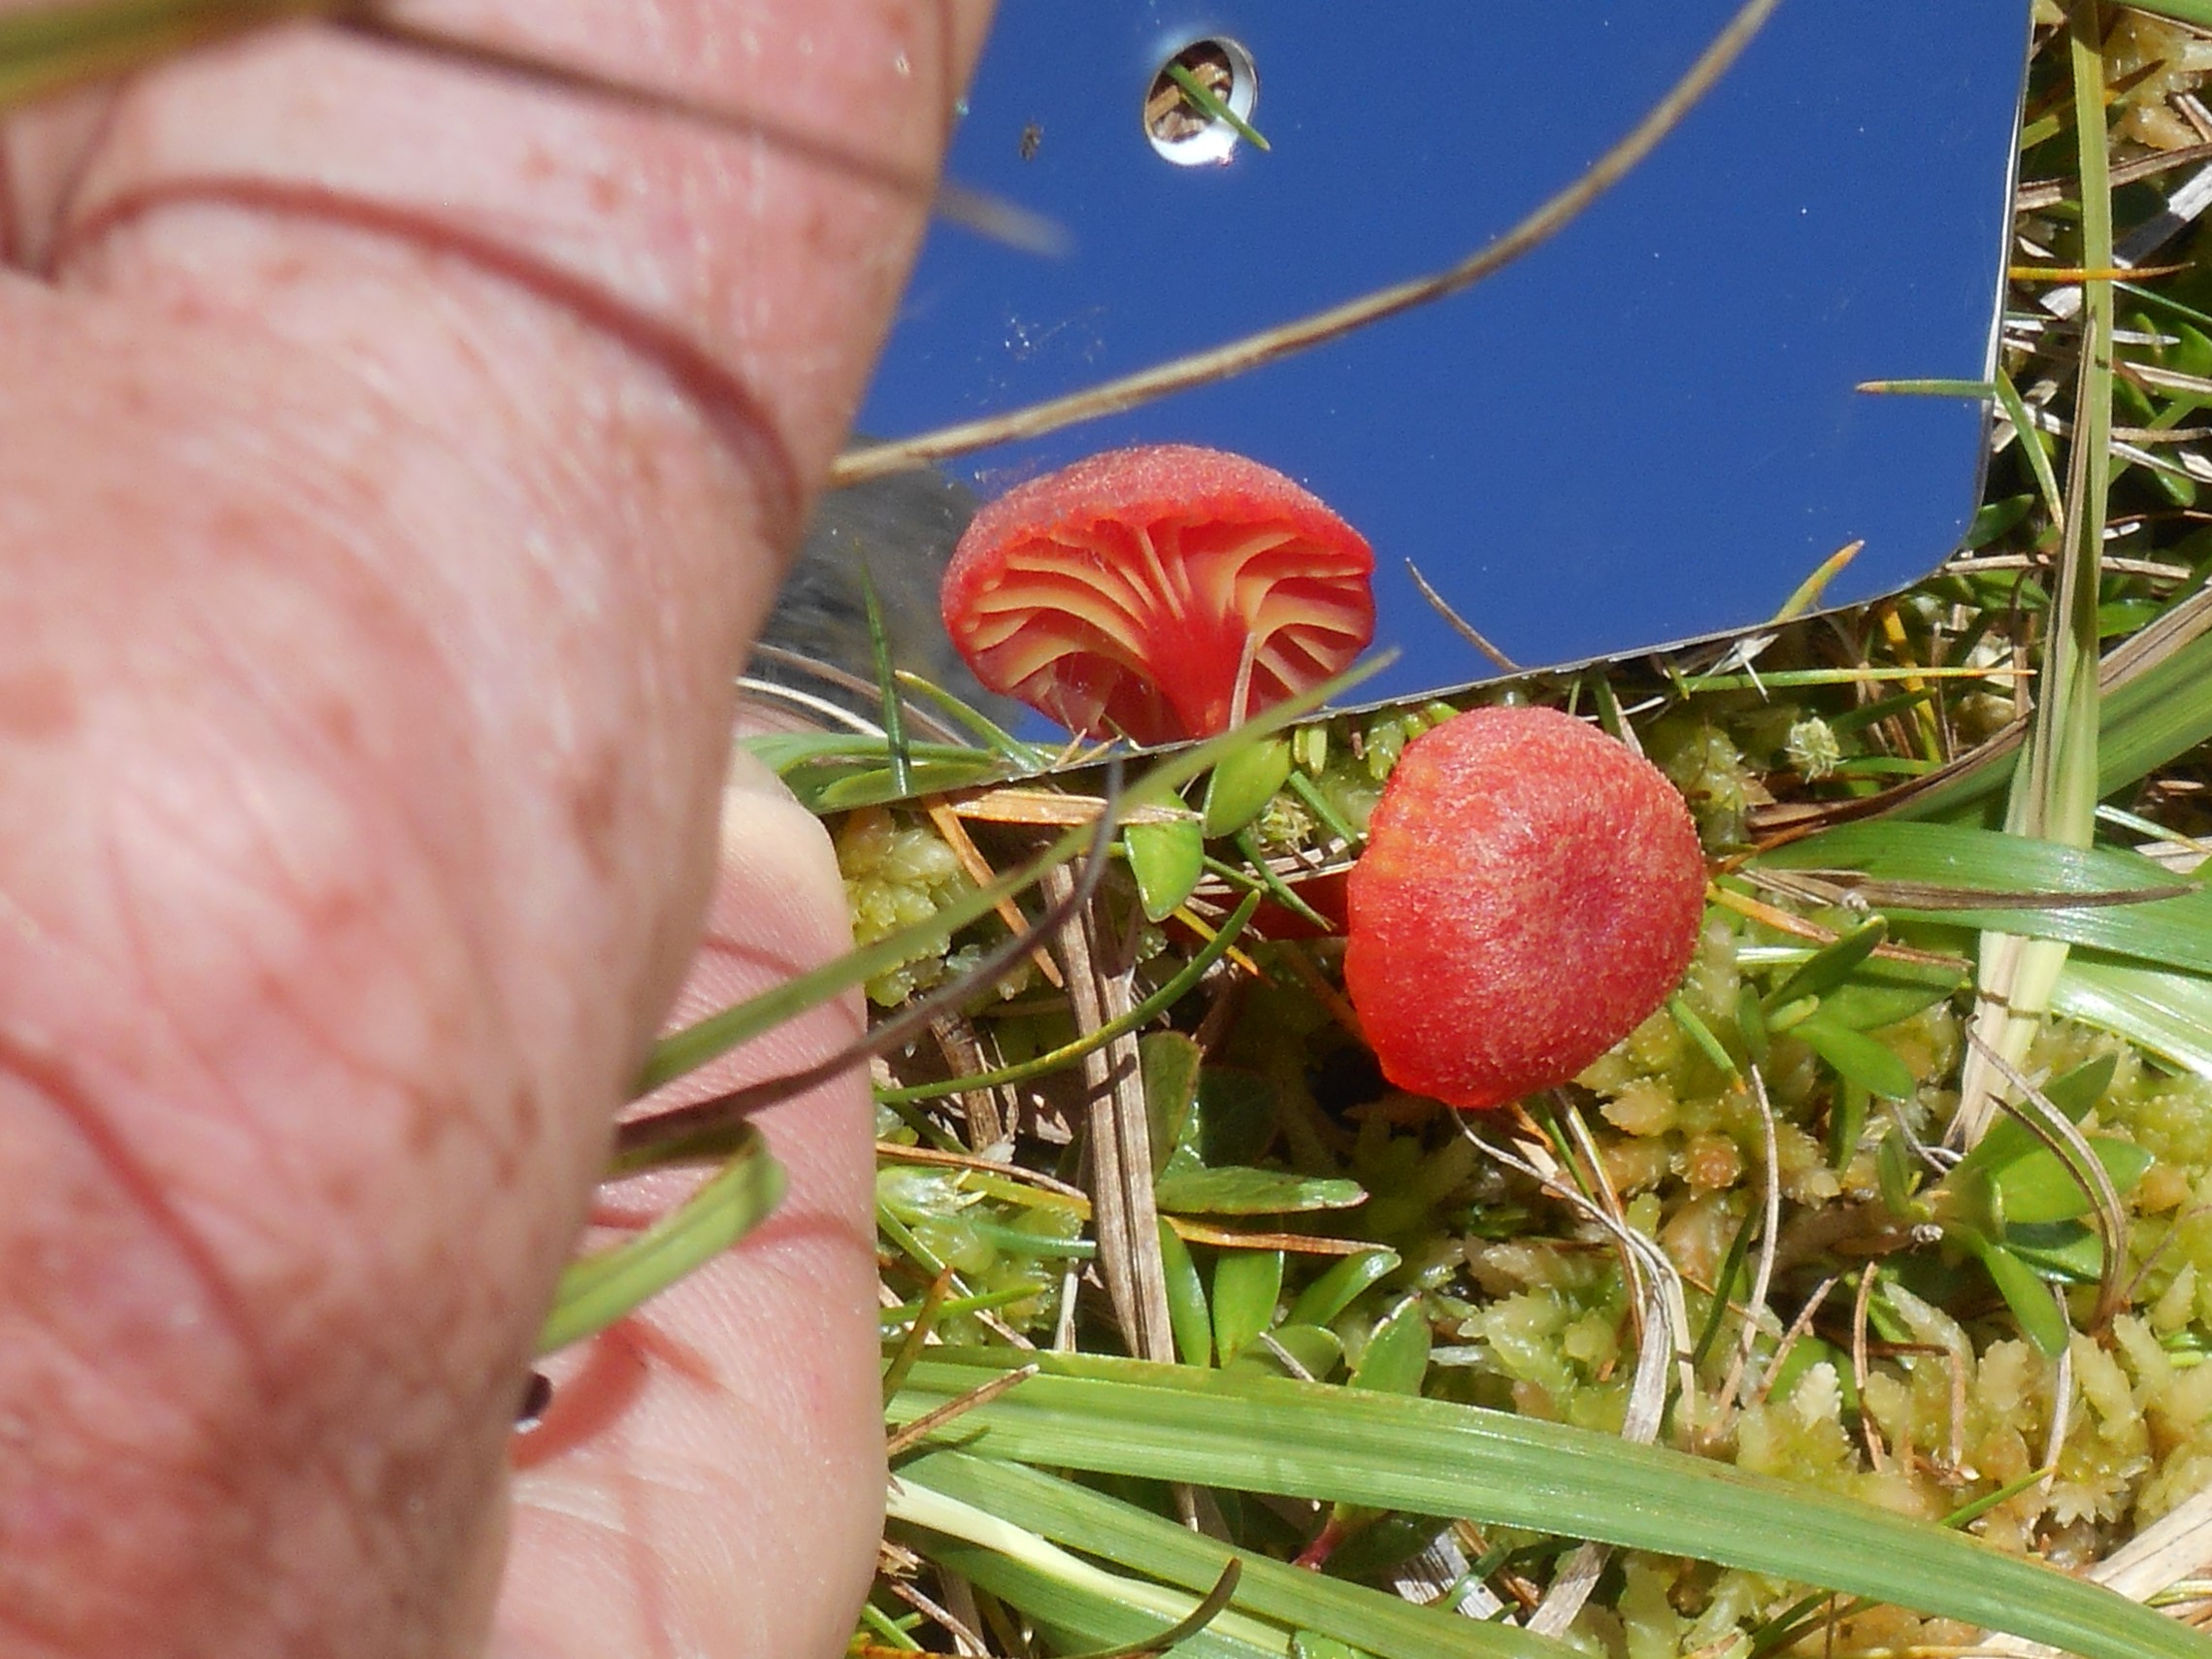
\includegraphics[width=8cm]{LakeManBivRecce7Jan2019Photo11}
   \captionof{figure}{Wax-cap fungi (\textit{Hygrocybe} sp)}
\end{flushright}
\end{minipage}
\end{figure}

On the final day we walked out to the river and crossed (unassisted this time) to the car and hence back home for lunch.  With the water levels prevalent at the time, the crossing was fine, although we did link up and prepare for a swim.

Despite the slow pace of the dog, we managed to stick to track times.  This was largely because Robyn carried him much of the way.  Methinks it'll be his last substantial walk, particularly as he didn't seem to enjoy it.

\begin{flushright}
Robyn, Peter and dog
\end{flushright}

\end{document}
